\chapter{Materials and Methods}\label{chap:materials-methods}
This chapter introduces the materials and datasets provided in the source paper \citep{Ferber2024}. We then describe how the data were preprocessed and explored, explain how the models were implemented, trained, and evaluated, and finally present the methods used to analyse model explainability.

\section{Data and Materials}\label{sec:method-data-materials}
As part of \citet{Ferber2024}, the authors have published a dataset of 1798 \glspl{subject} running or walking on a treadmill captured using multi-camera 3D \gls{mocapsys}. The dataset is composed of raw 3D marker data of each \gls{session}, descriptive biomechanical variables derived from the marker data for each session and demographic and anthropometric metadata of the subjects. Additionally, the matlab code for the preprocessing of the data, the calculation of the kinematic variables and tutorial notebooks that help lustrate how to use their library and read the data from the folder structure are also provided. Although both walking and running data is provided, we have used exclusively running data. From this point onwards, walking data is ignored for brevity.

\subsection{Measurement protocol}\label{subsec:measurement-protocol}
The complete measurement protocol is described in \citet{Ferber2024}. In this subsection, we provide a summary of the aspects that are most relevant for the methods and analyses presented in this thesis.

The raw marker data was collected using high-speed optoelectronic infrared-based motion capture cameras (MX3/Bonita, Vicon, Oxford, UK) were used to record the position of 9 mm spherical retro-reflective markers attached to anatomical landmarks of the subjects at either 120 Hz or 200 Hz. Depending on the lab, eight or three cameras were used. Below we list and describe the three sets of markers that were used.
\begin{itemize}
    \item \textbf{Core}: Markers attached to the following anatomical landmarks: medial and lateral malleoli, medial and lateral femoral condyles, and greater trochanters.
    \item \textbf{Additional}: Markers attached to the following anatomical landmarks: bilateral 1st and 5th metatarsal heads, distal aspect of the shoe, tibial tuberosity, anterior superior iliac spines, and iliac crests;
    \item \textbf{Clusters}: 3 or 4 markers placed on rigid shells attached to the following anatomical landmarks: sacrum, bilateral thigh and shank, and posterior aspect of both shoes.
\end{itemize}

During the recording of the sessions of all 1798 subjects the 'core' and 'cluster' set of markers were used. The additional set was only used during the recording of the sessions of 1082 subjects. Figure \ref{fig:marker_position} shows the lower body of a subject and the three sets of markers.

\begin{figure}[ht]
    \begin{centering}
    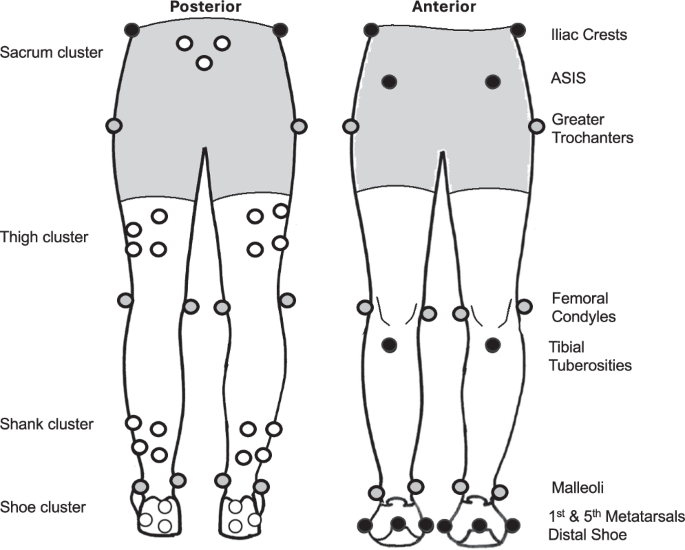
\includegraphics[width=0.5\columnwidth]{images/billateral_marker_position.png}
    \par\end{centering}
    \caption{Position of markers on the subjects. Grey markers correspond to core set of markers set, black to additional set and white to the clusters set.}
    \label{fig:marker_position}
\end{figure}

% TODO: Explain the recording procedure: Warm up, duration, discard, etc...

\subsection{Dataset Description}\label{subsec:method-dataset-description}
As described above, the dataset contains two complementary components: (i) session-level metadata stored as tabular files, and (ii) motion-capture marker data together with derived kinematic variables per session. Below we describe each component and list the variables that are available for analysis.

\paragraph{Metadata File (tabular)} The metadata file is provided as a CSV file: \texttt{run\_data\_meta.csv}. Each row corresponds to a single treadmill session recorded for a subject. It contains anthropometric and demographic variables.
\begin{itemize}
    \item \texttt{sub\_id}: Unique subject identifier.
    \item \texttt{datestring}: Session recording date.
    \item \texttt{filename}: Session filename used to locate the marker json file for the session.
    \item \texttt{speed\_r}: Treadmill belt speed (m/s).
    \item \texttt{age}: Subject's age (years).
    \item \texttt{Height}: Body height (cm).
    \item \texttt{Weight}: Body weight (kg).
    \item \texttt{Gender}: Subject gender.
    \item \texttt{DominantLeg}: Dominant leg (Left/Right/Ambidextrous).
    \item \texttt{InjDefn}: Injury severity reported by the subject choosing between 4 options: (1) No Injury, (2) Continuing to train in pain, (3) Training volume/intensity affected, (4) Minimum of two workouts missed in a row.
    \item \texttt{InjJoint}, \texttt{InjSide}, \texttt{SpecInjury}, \texttt{InjDuration}: Primary injured joint, side (Left/Right), Specific injury diagnosis from medical professional, and for how long has the subject had the injury.
    \item \texttt{InjJoint2}, \texttt{InjSide2}, \texttt{SpecInjury2}: Secondary injury information (if applicable).
    \item \texttt{Activities}: Subject reported athletic activities performed on a regular basis.
    \item \texttt{Level}: Self-reported level of athletic activity (recreational/competitive).
    \item \texttt{YrsRunning}: Number of years subject has been running on a regular basis.
    \item \texttt{RaceDistance}: Preferred race distance.
    \item \texttt{RaceTimeHrs}, \texttt{RaceTimeMins}, \texttt{RaceTimeSecs}: Preferred race distance best time.
    \item \texttt{YrPR}: Year of preferred race distance personal best time.
    \item \texttt{NumRaces}: Number of races completed per year.
\end{itemize}

\paragraph{Marker and descriptive biomechanical data (Hierarchical)} For each session, 3D positions of reflective markers and descriptive variables derived from those markers are provided as json files. One file per session.
\begin{itemize}
    \item \textbf{Recording frequency} Frequency of the recording in Hertz (Hz). Either 120 Hz or 200 Hz depending on the lab.
    \item \textbf{Joint Marker Neutral}: 3D coordinates of the individual markers of the core and additional marker sets while the subject is standing in neutral position.
    \item \textbf{Cluster Marker Neutral}: 3D coordinates of the individual markers in the cluster marker set while the subject is standing in neutral position.
    \item \textbf{Dynamic Marker data}: 3D coordinates at each of the frames of the recording for the individual markers in the cluster marker set.
    \item \textbf{Descriptive biomechanical variables}: Set of 77 variables derived from the 3D coordinates Marker data. Calculated for Left and Right side of the body.
\end{itemize}

It must be noted that \texttt{Joints} and \texttt{Neutral} coordinates do not represent the true anatomical centres, only the centres of the markers on the skin of the subject.
Only 33 of the 77 descriptive biomechanical variables are populated per side, the rest all contain 0 for all values of all sessions, this totals 66 populated descriptive variables in total. Table \ref{tab:met-desc-variable-init} describes the variable set per side.

\begin{table}[ht]
    \centering
    \caption[Populated Descriptive Variables Summary]{Summary of the Descriptive Biomechanical Variables that are populated\label{tab:met-desc-variable-init}}
    \begin{tabular}{lp{0.6\textwidth}}
    \hline
    \textbf{Variable} & \textbf{Category} \\
    \hline
    Step width (m) & Temporal-spatial \\
    Stride rate (steps/min) & Temporal-spatial \\
    Stride length (m) & Temporal-spatial \\
    Swing time & Temporal-spatial \\
    Stance time & Temporal-spatial \\
    Peak drop angle & Pelvis kinematics \\
    Drop excursion & Pelvis kinematics \\
    Dorsiflexion peak angle & Ankle kinematics \\
    Ankle Eversion peak angle & Ankle kinematics \\
    Ankle Rotation peak angle & Ankle kinematics \\
    Ankle Eversion excursion & Ankle kinematics \\
    Ankle Rotation excursion & Ankle kinematics \\
    Ankle Eversion \% of stance & Ankle kinematics \\
    Knee Flexion peak angle & Knee kinematics \\
    Knee Adduction/abduction peak angle & Knee kinematics \\
    Knee Rotation peak angle & Knee kinematics \\
    Knee Adduction/abduction excursion & Knee kinematics \\
    Knee Rotation excursion & Knee kinematics \\
    Hip Extension peak angle & Hip kinematics \\
    Hip Adduction peak angle & Hip kinematics \\
    Hip Rotation peak angle & Hip kinematics \\
    Hip Adduction excursion & Hip kinematics \\
    Hip Rotation excursion & Hip kinematics \\
    Foot progression angle & Foot kinematics \\
    Heel-strike angle & Foot kinematics \\
    Medial heel whip excursion from toe-off & Foot kinematics \\
    Ankle eversion peak velocity & Joint velocities \\
    Ankle rotation peak velocity & Joint velocities \\
    Knee adduction peak velocity & Joint velocities \\
    Knee abduction peak velocity & Joint velocities \\
    Hip abduction peak velocity & Joint velocities \\
    Knee rotation peak velocity & Joint velocities \\
    Hip rotation peak velocity & Joint velocities \\
    Pelvic drop peak velocity & Joint velocities \\
    Pronation onset \% of gait cycle & Foot timing \\
    Pronation offset \% of gait cycle & Foot timing \\
    Vertical oscillation (mm) & Vertical oscillation \\
    \hline
    \end{tabular}
\end{table}

All descriptive variables follow the interpretations described in \citet{Bartlett2014}. Unless specified explicitly in the table, the units are degrees for angles and excursions, and degrees/s for joint velocities. Excursions are also commonly known as range of motion (ROM) in the literature. 
% TODO: Explain important biomechanical concepts like dorsiflexion, eversion, etc...


\subsection{Code Description}\label{subsec:method-code-description}
Python was the main language used in this project, although several scripts were implemented in \GLS{matlab} for the data acquisition and extraction stages. Matlab was also used to preprocess the dataset, following the procedure described in the source paper. All code created for this project and used to generate the reported results has been made publicly available for reproducibility \cite{Zapater_Reig_Running_Injury_Clinic_2025}.  

The MATLAB reference implementation published with the dataset in \citet{Ferber2024} was employed as part of this work. The corresponding MATLAB scripts have been included in the repository under the \texttt{supplemental\_material} folder for consultation.  

The following assets are the most relevant components of the repository:  

\paragraph{Notebooks}  
\Gls{jupyter} notebooks used during development. These capture the iterative process across the different phases of the project and the reporting of results.

\paragraph{\texttt{core} Package}  
Python package containing the core functionality used in the notebooks. It includes classes, functions, and constants to orchestrate data extraction, preprocessing, feature engineering, model training, and evaluation.  

\paragraph{\texttt{gait\_kinematics.m}}  
Script provided with the source paper. It calculates joint angles and angular velocities from the \texttt{Dynamic Marker Data}, \texttt{Joint Marker Neutral}, and \texttt{Cluster Marker Neutral} files. Anatomical segment coordinate systems are constructed from the neutral marker data, segment motion is tracked using the dynamic marker data, and XYZ Cardan joint angles and angular velocities are computed. The script returns:  
\begin{itemize}
    \item \texttt{Angles}: per-frame joint/segment angles for the left/right ankle, knee, hip, as well as foot and pelvis segments (degrees).
    \item \texttt{Velocities}: per-frame angular velocities for the same structures (deg/s).
    \item \texttt{jc}: estimated joint centre positions (pelvis, hips, knees, ankles).
\end{itemize}

\paragraph{\texttt{gait\_steps.m}}  
Script also provided with the source paper. It calculates descriptive biomechanical variables from the \texttt{Dynamic Marker Data}, \texttt{Cluster Marker Neutral}, \texttt{Angles}, and \texttt{Velocities}. The script returns:  
\begin{itemize}
    \item \texttt{event}: gait cycle events by side (touchdown, mid-stance, toe-off, heel whip).
    \item \texttt{Descriptive biomechanical variables}: as defined in Table~\ref{tab:met-desc-variable-init}.
\end{itemize}

\paragraph{\texttt{processing\_source\_data.m}}  
Script implemented for this project to process the metadata file and marker-data JSON files. Joint angles, joint angular velocities and cycle events are computed by calling \texttt{gait\_kinematics.m} and \texttt{gait\_steps.m}. The outputs are converted into tabular format for the exploratory data analysis (EDA) stage.


\subsection{Data Extraction}\label{subsec:data-extraction}

The script \texttt{processing\_source\_data.m} was executed to process the raw dataset. Out of 2506 recorded sessions (with some subjects contributing multiple sessions), 2487 were processed successfully, of which 1813 contained valid running data. Sessions without running data or those where MATLAB preprocessing failed were excluded.  

The outputs consist of time-series data for markers, joint angles, joint angular velocities, and detected gait cycle events with their corresponding frame indices. These outputs were further processed using the \texttt{pandas} and \texttt{kinetics-toolkit} Python packages to combine the event information with the time-series data.  

Figure \ref{fig:data-ext-marker-velo-angle-ts} illustrates an example from a single session, showing the raw marker data for one marker in the left shank cluster together with the corresponding joint angle and angular velocity for the left knee. Figure \ref{fig:data-ext-l-knee-angle-events} shows frames 500--1000 of the left knee angle, annotated with the touchdown and toe-off events. Figure \ref{fig:data-ext-marker-3d} provides a 3D representation of a frame with the full marker set.  

In addition to the time-series data, the script also generates a set of 33 descriptive variables. These variables are equivalent to those stored in the JSON files of the source dataset. To validate the execution of \texttt{processing\_source\_data.m}, the generated variables were compared against the source dataset. All variables matched within a relative tolerance of $1 \times 10^{-9}$, except for 35 values of \texttt{speed\_r}, which differed by $9 \times 10^{-2}$. This deviation is negligible when measuring human running speed in m/s and confirms that the execution was successful. The computed set of descriptive variables was discarded in favour of the original dataset variables, which included 1832 samples. The resulting data were therefore considered ready for the exploratory data analysis stage.

\begin{figure}[ht]
    \centering
    \begin{minipage}[t]{0.48\textwidth}
        \centering
        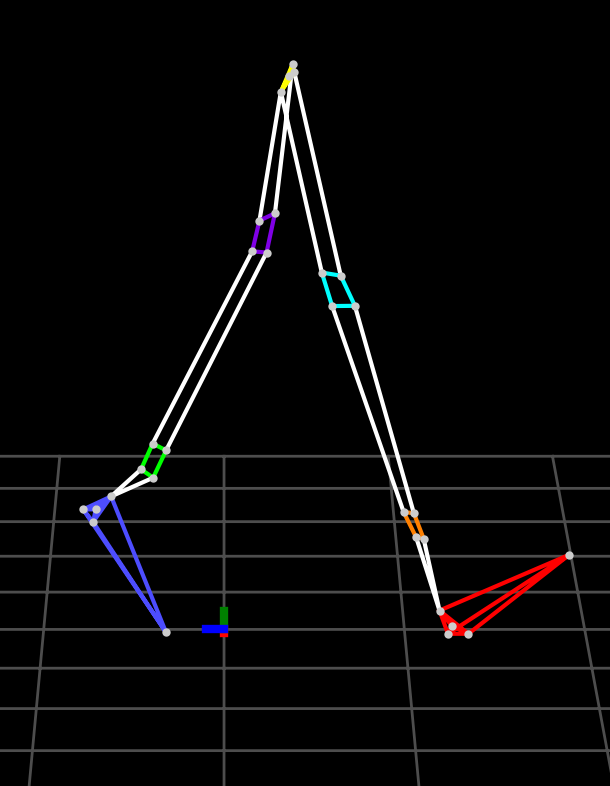
\includegraphics[width=\textwidth]{images/ex_3d_marker.png}
        \caption{3D representation of a frame with all marker data. Connecting lines have been added between markers. The left foot is coloured blue and the right foot red. From top to bottom: pelvis, left/right thigh, left/right shank, and left/right foot.}
        \label{fig:data-ext-marker-3d}
    \end{minipage}
    \hfill
    \begin{minipage}[t]{0.48\textwidth}
        \centering
        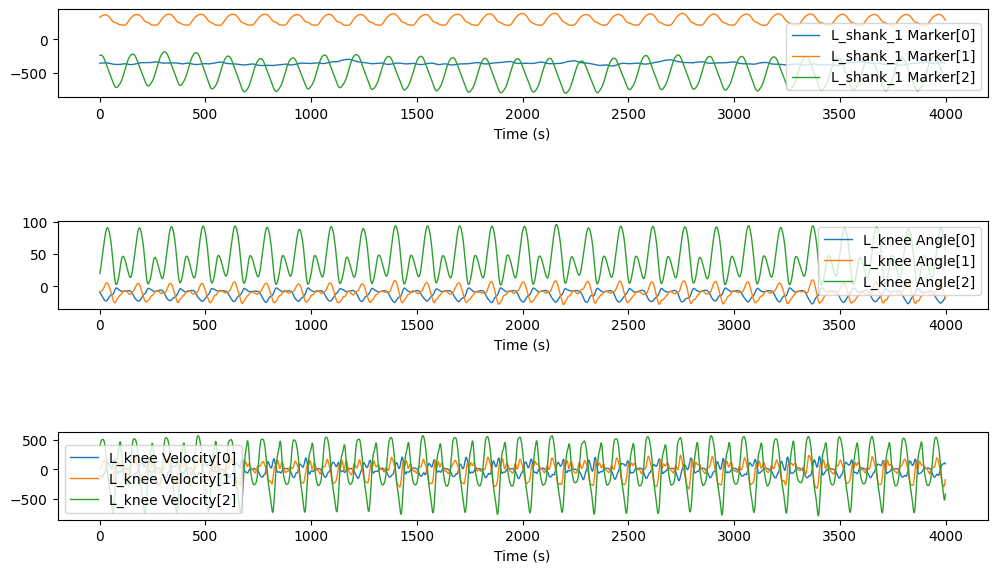
\includegraphics[width=\textwidth]{images/ex_marker_angle_vel_ts.png}
        \caption{Example time series from a single session showing the first left shank marker, left knee angle, and left knee angular velocity across the three axes: [0] X, [1] Y, [2] Z.}
        \label{fig:data-ext-marker-velo-angle-ts}
    \end{minipage}
\end{figure}

\begin{figure}[ht]
    \centering
    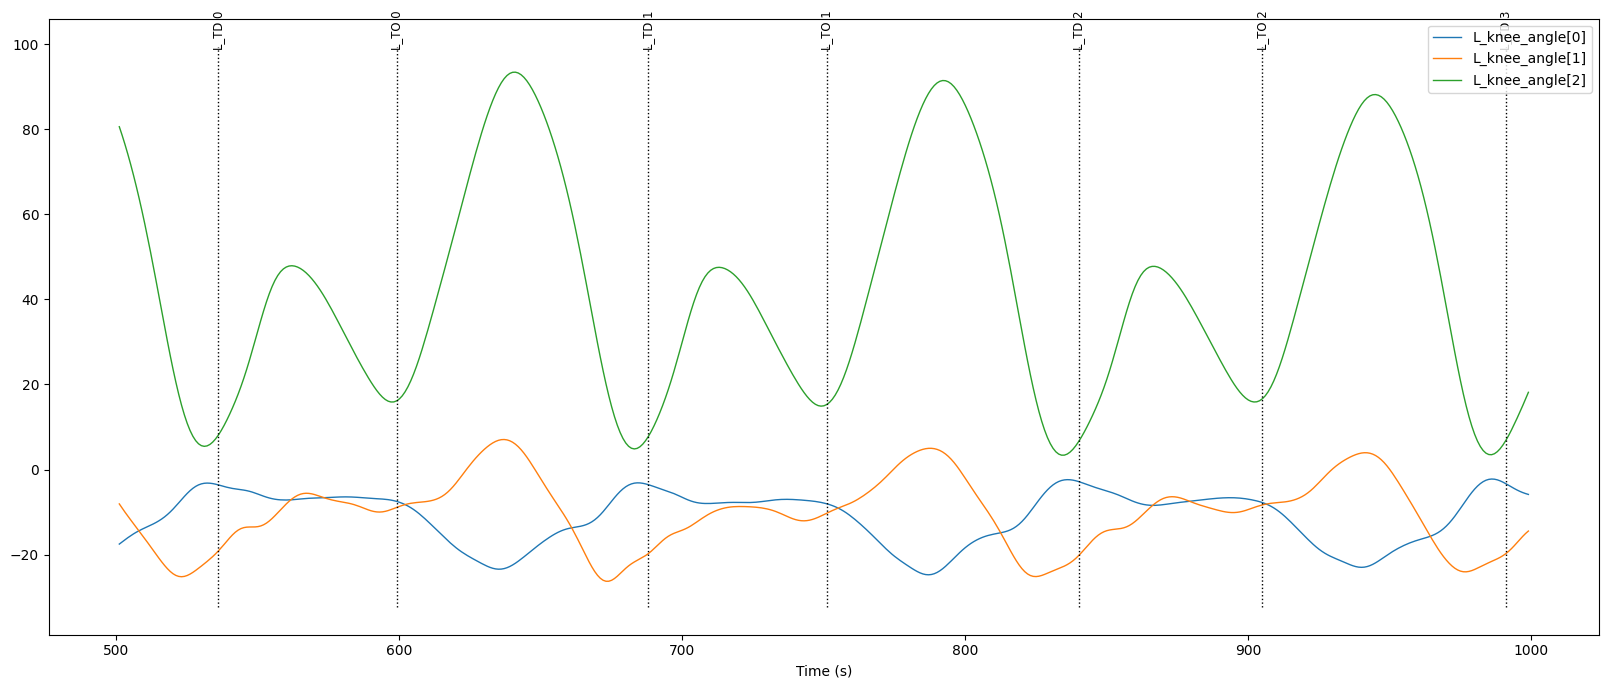
\includegraphics[width=0.5\columnwidth]{images/ex_l_knee_angle_events.png}
    \caption{Frames 500--1000 of the left knee angle (three axes: [0] X, [1] Y, [2] Z), annotated with touchdown (\(L\_TD\)) and toe-off (\(L\_TO\)) events.}
    \label{fig:data-ext-l-knee-angle-events}
\end{figure}


% TODO: End with a summary of the tabular and time-series data that we have extracted?

\section{Exploratory Data Analysis (EDA)}\label{sec:method-eda}
% -- Exploration → Extraction → Preparation, with concrete checks and figures:
% -- Tabular data Exploration (sanity and distributions)
% -- Dataset inventory (sessions per runner, class prevalence per runner, cycles/session).
% -- Missing-ness map (metadata \& signals); strategy preview (drop/impute).
% -- Outliers: per-joint angle/velocity ranges, z-score >3 heat-map by runner (flag sensors/markers).
% -- Dimensionality previews: PCA/t-SNE to see separability.
As discussed on the previous section, we have two main types of data available:

\begin{itemize}
    \item \textbf{Tabular datasets}
    \begin{itemize}
        \item Session metadata, a set of anthropometric and demographic variables.
        \item Descriptive variables, a engineered set of biomechanical variables derived from the joint angles and angular velocities.
    \end{itemize}
    \item \textbf{Time-series datasets}
    \begin{itemize}
        \item Joint angles derived from the marker data.
        \item Joint angular velocities derived from the marker data.
    \end{itemize}
\end{itemize}

Given the difference in structure of both groups of datasets we need to apply different techniques and methods when working with them. Below we will discuss each of them separately.

\subsection{Tabular dataset}\label{subsec:method-tabular-dataset}
The tabular datasets contain a row for each of the 1832 recordings of running sessions. There are 1402 distinct runners within those sessions, with 209 of them having more than 1 session recorded. There are 19 more sessions compared to the time-series datasets due to the errors during data extraction. Still, we will use the full tabular dataset, for the tasks that require only tabular data, since there are no data quality issues with the tabular data of those sessions.

\paragraph{Standardisation of variables:}
The values of nominal categorical variables with less than 100 categories have been mapped to a code that is easier to work with(no spaces, no special characters and restricted length), and we have consolidated categories that refer to the same code but were written slightly differently (i.e. meniscal tear-lateral and meniscal tear lateral).

For nominal categorical variables with more than 100 categories that are likely a free text input for the subjects like \texttt{Activities}, we Convert to lowercase, remove leading and trailing spaces, replace non-standard separators with comma, replace multiple spaces with single space, replace multiple commas with single comma.

For ordinal categorical values, we have introduced both a code and a numerical representation so that we can choose what to use depending on the task.
Quantitative variables have been left unchanged, standardisation and normalization has been left for a later stage.

All values that do not fall into a defined category or an accepted value for the data-type are considered as missing value and are converted to None. This is saved as "" when saving the dataset to CSV format.

> TODO: Expan each of the points and add visualization if needed.

Key points regarding the distributions of the columns:
\begin{itemize}
    \item The male/female distribution is balanced (exact percentage to be reported), with an additional "unknown" category present.
    \item The \texttt{DominantLeg} variable is skewed towards the right leg, as expected; there are few ambidextrous cases.
    \item The distributions of \texttt{SpecInjury} and \texttt{InjDefn} are noteworthy and should be reported.
    \item The "Level" variable (recreational vs. competitive) is skewed towards recreational runners.
    \item There is little longitudinal data: only 30 sessions (2.1\%) are at least one month apart.
\end{itemize}

\paragraph{Data quality and outlier detection} 

During inspection of the dataset, several inconsistencies were identified. In some cases, the level of athletic activity (\texttt{Level}), the reported dominant leg (\texttt{DominantLeg}), and the injury descriptors (\texttt{SpecInjury} and \texttt{InjDefn}) changed across sessions for the same subject. These cases were considered plausible and interpreted as part of the natural variability of the dataset. No indication was found in the source paper that such cases should be regarded as data quality issues, and they were therefore left unchanged.  

One case was found in which the reported age differed by ten years between two sessions, which exceeds the duration of the study. To investigate, the entire dataset was checked for inconsistencies between reported age and the time difference between sessions. Two problematic cases were identified:  
\begin{itemize}
    \item Subject 100234 was recorded as 40 years old in the first session and 43 years old one year later. In this case, the age in the second session was corrected to 41.  
    \item Subject 200375 was recorded as a 27-year-old female in one session and as a 50-year-old male in the next. This inconsistency suggests that the sessions belong to different individuals. A new synthetic subject identifier (300375) was therefore created, and the second session was reassigned to this new subject. The total number of sessions remained unchanged, but the number of unique subjects increased by one.  
\end{itemize}

Additional inconsistencies were found in the injury variables. In many sessions, \texttt{SpecInjury} was empty while \texttt{SpecInjury2} contained information. These cases were treated as input errors: when \texttt{SpecInjury} was missing and \texttt{SpecInjury2} was populated, the value of \texttt{SpecInjury2} was taken as the primary injury. A subject was assumed to have no primary injury in a session only if both fields were empty.  

All columns in the metadata were inspected for implausible values. Table \ref{tab:met-outlier-range} summarises the range thresholds used for outlier detection. Values outside of these ranges were considered unrealistic and replaced with \texttt{None}. For example, ages of 255 years, heights of 999~cm, weights of 1564~kg, injury durations of 30,000 days (82 years), and years running of 999 were identified as outliers and removed. These extreme values were detected visually using box plots and validated against plausible ranges for human adults.  

\begin{table}[h!]
    \centering
    \caption[Outlier detection range for tabular data]{Summary of outlier detection ranges for key variables.\label{tab:met-outlier-range}}
    \begin{tabular}{lcc}
        \hline
        \textbf{Variable} & \textbf{Min} & \textbf{Max} \\
        \hline
        Age & 18.0 & 73.0 \\
        Height (cm) & 120.0 & 196.5 \\
        Weight (kg) & 42.5 & 176.0 \\
        Injury duration (days) & 0.0 & 176.0 \\
        Years running & 0.0 & 54.0 \\
        \hline
    \end{tabular}
\end{table}


\paragraph{Merging metadata and biomechanical variables}
We decided to introduce a surrogate key "id" that can be used across datasets to identify each sample uniquely. One sample is a session. The surrogate key is the concatenation of subject id with the filename in uppercase i.e. \"100001\_20110531T161051\". We use this column to join both datasets by "id".

% TODO: List all variables available? Maybe better on a Apendinx?

\paragraph{Missing values:}
Missing data:
<table> Missing data, table with columns with most missing values after cleaning
As expected \texttt{SpecInjury2}, \texttt{InjJoint2} and \texttt{InjSide2} has the most missing values, it is only populated when a subject has two injuries reported. If it only has 1, then it will be empty. There are data quality issues with those columns, because they missing values \% do not match.

Columns with more than 30\% of missing values will not be used for modelling.


\paragraph{Definition of Injury status}
Definition of Injury: the dataset does not contain a column that marks injury, we have two columns with relevant information: \texttt{SpecInjury} and \texttt{InjDefn}. The former is the injury reported by a medical expert and the latter is the injury severity self-reported by the patient. Identifying a positive injury status should be easy, but we have found some edge cases where a runner reported no injury and the medical expert diagnosed an injury, and the inverse scenario too.

<Image with distribution of InjDefn> 
<Image with visualization of injuries - Word map?> 


TODO: What conclusions of the exploration of injury data can be derived?
TODO: Healthy vs injured distribution.


\subsection{Time-series dataset}\label{subsec:method-ts-dataset}

% -- Time-series data Exploration:
% -- Visuals: overlay of 20 random stance cycles per class; Markers, Angles, Velocities, ...
% -- Analysis of curves
% -- Extraction (curve-level descriptors)


% -- Preparation (decisions fixed before modelling)

% -- Group-aware split policy (runner-level), ensuring no cycle leakage across folds.
% -- Class-imbalance diagnostics (AUC-PR baseline, per-runner prevalence plots).
% -- Filtering rules for cycles/sessions (min cycles per session, quality thresholds).

% -- Final feature set(s) to carry forward (e.g., summaries, PC scores, raw curves for DL)

% TODO: Maybe we keep outliers and filering here?



\section{Pre-processing}\label{sec:method-preprocessing}
-- Tabular:
    -- filtering, subject identification, outliers, cleaning, etc..
    -- Final dataset creation -> Give name to track

-- Time-series:
    -- Extraction of angles and angular velocities as mentioned in literature.
    -- Extraction of events
    -- Combination of events and TS
    -- Cycle Segmentation and normalization -> Reference papers either here or in SOTA.

\subsection{Feature Engineering}\label{subsec:method-feature-engineering}
-- Transformations and feature extraction
    -- Dominant Leg -> VIF reduction
    -- Obtaining a representative curve
        -- Curve registration attempt and Actual result

-- Feature selection:
    -- MRMR for feature selection

\subsection{Feature Selection}\label{subsec:method-feature-selection}
-- Transformations and feature extraction
    -- Dominant Leg -> VIF reduction
    -- Obtaining a representative curve
        -- Curve registration attempt and Actual result

-- Feature selection:
    -- MRMR for feature selection

% \subsection{Tabular Data}\label{subsec:method-tabular-data}
% -- Correlations mutual information, ...
% -- Collinearity: PCA, VIF, ...
% -- Left-right features - Dominant leg extraction
% -- Collinearity reduction

% \subsection{Timeseries Data}\label{subsec:method-timeseries-data}
% -- Segmentation: TD/TO, stance, swing, ...
% -- Normalisation/standardisation

\subsection{Final Feature Sets}\label{subsec:method-final-feature-sets}
-- Summary of the feature by dataset.

\section{Models}\label{sec:method-models}
\subsection{Baseline (Tabular)}\label{subsec:method-baselines}
\subsection{Deep Learning}\label{subsec:method-deep-learning}
-- Unilateral LSTM
-- Bilateral LSTM
-- Multimodal
-- TMAG
-- MC DCNN

-- Add special tuning for class imbalance, etc...
-- Architecture choices (hyperparameters, etc...)
-- class imbalance, oversampling, etc... TBD Where to put this? -> Explain in the models that used it. We will give results for each option individually.

\section{Evaluation Protocol}\label{sec:method-evaluation-protocol}
-- The blueprint before we run anything.
-- Questions/Hipothesis, grouping, leakage, validation scheme (group-aware train/val/test)
-- Evaluation protocol -> Measurements, statistics. How are we scoring the experimentriment. (Primary, Secondary metric, Threshold rule, ...).
-- Significance Tests. How do we know something is "Better" (DeLong's test)?
-- CI 95 \%
-- Research questions (RQs), validation scheme (group-aware train/val/test), splits, primary/secondary metrics.
-- Justify the choices , but do not present any results yet...

% \subsection{Evaluation Metrics}\label{subsec:method-evaluation-metrics}
% - AUC ROC + PR for class imbalance + Macro F1 score for threshold.

\subsection{Training and Validation Strategy}\label{subsec:method-training-validation-strategy}
-- Train, test, validation split.
-- Group-aware split policy (runner-level), ensuring no cycle leakage across folds.
-- Class-imbalance diagnostics (AUC-PR baseline, prevalence).

\subsection{Hyperparameter Tuning}\label{subsec:method-hyperparameter-tuning}
-- Grid search, random search, ...
-- Cross-validation, nested cross-validation, ...
-- Early stopping, ...
-- Hyperparameter tuning strategy.


% TODO: Add Traing and use of Cross Validation


\section{Explainability}\label{sec:method-explainability}
<Draft> This project would have been set up differently if the sole goal had been to build and deploy an injury detection model. In that case, explainability would mostly be used just to debug the model, and the focus would shift toward making data collection easier, choosing an efficient architecture, and reducing resource use. In our case, though, explainability is central: a deep learning model with an AUC-ROC of 0.7 doesn't add much value if it remains a black box.

To get the most out of this work, we used both intrinsic methods and Explainable AI (XAI) techniques, as in \cite{FuentesJimnez2025}, to make the model's decisions more transparent.

\subsection{Intrinsic Explainability}\label{subsec:method-intrinsic-explainability}
- Random Forest, linear regression, etc...
-- Pros, Cons, etc..
-- what affects them?

\subsection{Post-hoc Explainability}\label{subsec:method-posthoc-explainability}
-- SHAPs, Saliency maps, feature permutation?



% \section{Reproducibility Assets}\label{sec:method-reproducibility}
% -- code repository structure, libraries, etc...
